\section{Selection Variables \label{sec:SelVar}}
The low velocity of HSCPs lead to two interesting detector signatures. The first is that the particles will arrive at the detector elements later than SM particles will.
The muon system, being the furthest detector element from the interaction point, has the largest timing difference. The measurement of the arrival time of particles in the
muon system is discussed in Ch.~\ref{sec:timing}. The \invbeta\ variable is used in the searches to discriminate between HSCPs and SM particles.

The second signature is the amount of ionization energy loss HSCP have in the inner tracker.
%that a slow moving HSCP will have a larger ionization energy loss in the silicon tracker than SM particles will.
The amount of the ionization energy lost per unit length, \dedx, is dependent on both the velocity of the HSCP and its charge as described by the Bethe-Bloch formula~\cite{PDG}.
The dependence of \dedx\  on charge goes as $Q^2$, meaning that even a $Q=2e$ HSCP will have four times as much energy loss as a SM particle.
The dependence on speed for particles with $0.1 < \beta < 1$, goes as $\sim 1/\beta^2$.
SM particles with momentum 10-1000 GeV will all have roughly the same $\dedx,$ ($\approx$ 3MeV/cm) and are often referred to as minimum ionizing particles (MIPs).

As in~\cite{Chatrchyan:2012sp}, two variables related to \dedx\ are calculated for each track. The first is \ih\ which is an estimator of the \dedx\ of the track.
The second is \ias\ which is a modified version of the Smirnov-Cramer-von Mises~\cite{Eadie, James} discriminant that checks
the probability that a MIP would produce a charge less than or equal to the charge of each of the hits
along the track. The discriminant peaks at zero for MIPs and approaches one for high-ionizing particles. 

%The last is \iasp\ which has the same form as \ias\ except
%the probability is that a MIP would produce a charge more than or equal to the charge of the hits, this variable is only used in the fractionally charged analysis.

An estimate of the mass $m$, assuming Q=1$e$, of a particle can be made from \ih\ and the momentum $p$ of a track. This is done by using Eq.~\ref{eq:MassFromHarmonicEstimator},
also from Ref.~\cite{Chatrchyan:2012sp},

\begin{equation}
I_h= K\cfrac{m^2}{p^2}+C.
\label{eq:MassFromHarmonicEstimator}
\end{equation}

with  $K=2.559 \pm 0.001$ MeV cm$^{-1}$ $c^2$ and
$C=2.772 \pm 0.001$ MeV cm$^{-1}$.

The last selection variable used in the analyses is transverse momentum.
HSCP would be produced by BSM theories that have a high energy scale, leading to the HSCP to be produced with much
more momentum than is typical for SM particles.
%Staus produced from the decay of heavier particles have high momentum due to the mass difference between the stau and the mother particle.
%For this reason the $p_T$ of the track is used as a third
%selection variable. 

The \muononly\ analysis uses the $p_T$ measurement coming from the muon system while the rest of the analyses use the measurement from the inner tracker.
$R-hadrons$ are unlikely to undergo a nuclear interaction while traversing the tracker so they would have the same electric charge at all points in the tracker.
While passing through the muon system however, R-hadrons will often undergo a nuclear interaction with the steel return yoke located between the muon stations
possibly causing the electric charge to change in the middle of the muon system. This behavior affects the reconstruction of the HSCP track.
%gh the inner tracker so the \tktof\ is relatively unaffected by this. However for the $p_T$ measurement from the muon system it can result in the $p_T$ of the
%HSCP to be overestimated.

CMS measures the curvature of a track which can then be used to determine the $Q/p_T$ of the track. A charge of $Q=1e$ is assumed in order to determine the $p_T$ of the track.
For $R-hadrons$ that can change their charge inside of CMS it can be the case that the average value of Q during its passage through the muon system does not equal one.
This effect has different consequences for the stop and gluino samples. 

A stop particle, specifically not an anti-stop, has a charge of $+(2/3)e$ and forms a $R$-hadron with either an anti-quark ($\tilde{t} \bar{q}$) or
two quarks  ($\tilde{t} q q$). Anti-quarks have a charge of $-(2/3)e$ or $+(1/3)e$ leading to $R$-hadrons with a charge
of either 0 or $+1e$. Quarks have a charge of either $+(2/3)e$ or $-(1/3)e$ which allows for
the creation of $R$-hadrons with a charge of 0, $+1e$, or $+2e$. Thus a stop $R$-hadron will always have a
positive charge or be neutral. For an anti-stop, the effect is reversed and the $R$-hadron will always have a
negative charge or be neutral.

For gluino $R-hadrons$ this statement does not hold true. Gluinos can hadronize into glue balls ($\tilde{g}g$), $R$-mesons ($\tilde{g} q \bar{q}$), or
$R$-baryons  with either quarks or anti-quarks ($\tilde{g} qqq$ or $\tilde{g} \bar{q}\bar{q}\bar{q}$),
allowing the charge of the $R$-hadron to range from $-2e$ to $+2e$. This leads to the
average charge of the $R$-hadron as it traverses the muon system to often be less than $1e$ and the $p_T$ value to be overestimated.

To observe this effect the function
$\Delta(Q/p_T)$ is defined in Equation~\ref{eq:deltaqopt}
\begin{equation}
\Delta(Q/p_T) = ((Q/p_T)_{Muon} - (Q/p_T)_{Inner})/(Q/p_T)_{Inner}
\label{eq:deltaqopt}
\end{equation}
where ``Muon'' refers to muon system track qualities and ``Inner'' refers to
inner track qualities. As the $p_T$ resolution in the tracker is an order of magnitude better than in the muon system, it is a sufficiently good approximation
of the true particle momentum. Figure~\ref{fig:MuOnlyInvPtDiff} shows the distribution of
$\Delta(Q/p_T)$ for tracks with inner track $p_T > 200$ GeV
for data and various HSCP signal samples.
A value of zero in this plot indicates the $p_T$ was reconstructed correctly
while negative one indicates the reconstructed $p_T$ approaches infinity.
The GMSB stau sample, which does not change charge,
has a distribution similar to data, though slightly wider.
The slight discontinuity at negative one is due to particularities of the reconstruction but only affects a small number of tracks.
The stop sample, which is not able to flip charge but merely to switch
between one sign and zero, is centered at zero but with a slightly wider
width than data or GMSB stau.
The gluino sample, which can flip charge, is centered closer to negative one meaning that
their reconstructed $p_T$ is normally larger than what is generated, sometimes
to a very large degree.  This effect causes further discrimination of gluino HSCP
from background Standard Model particles.

\begin{figure}
 \begin{center}
  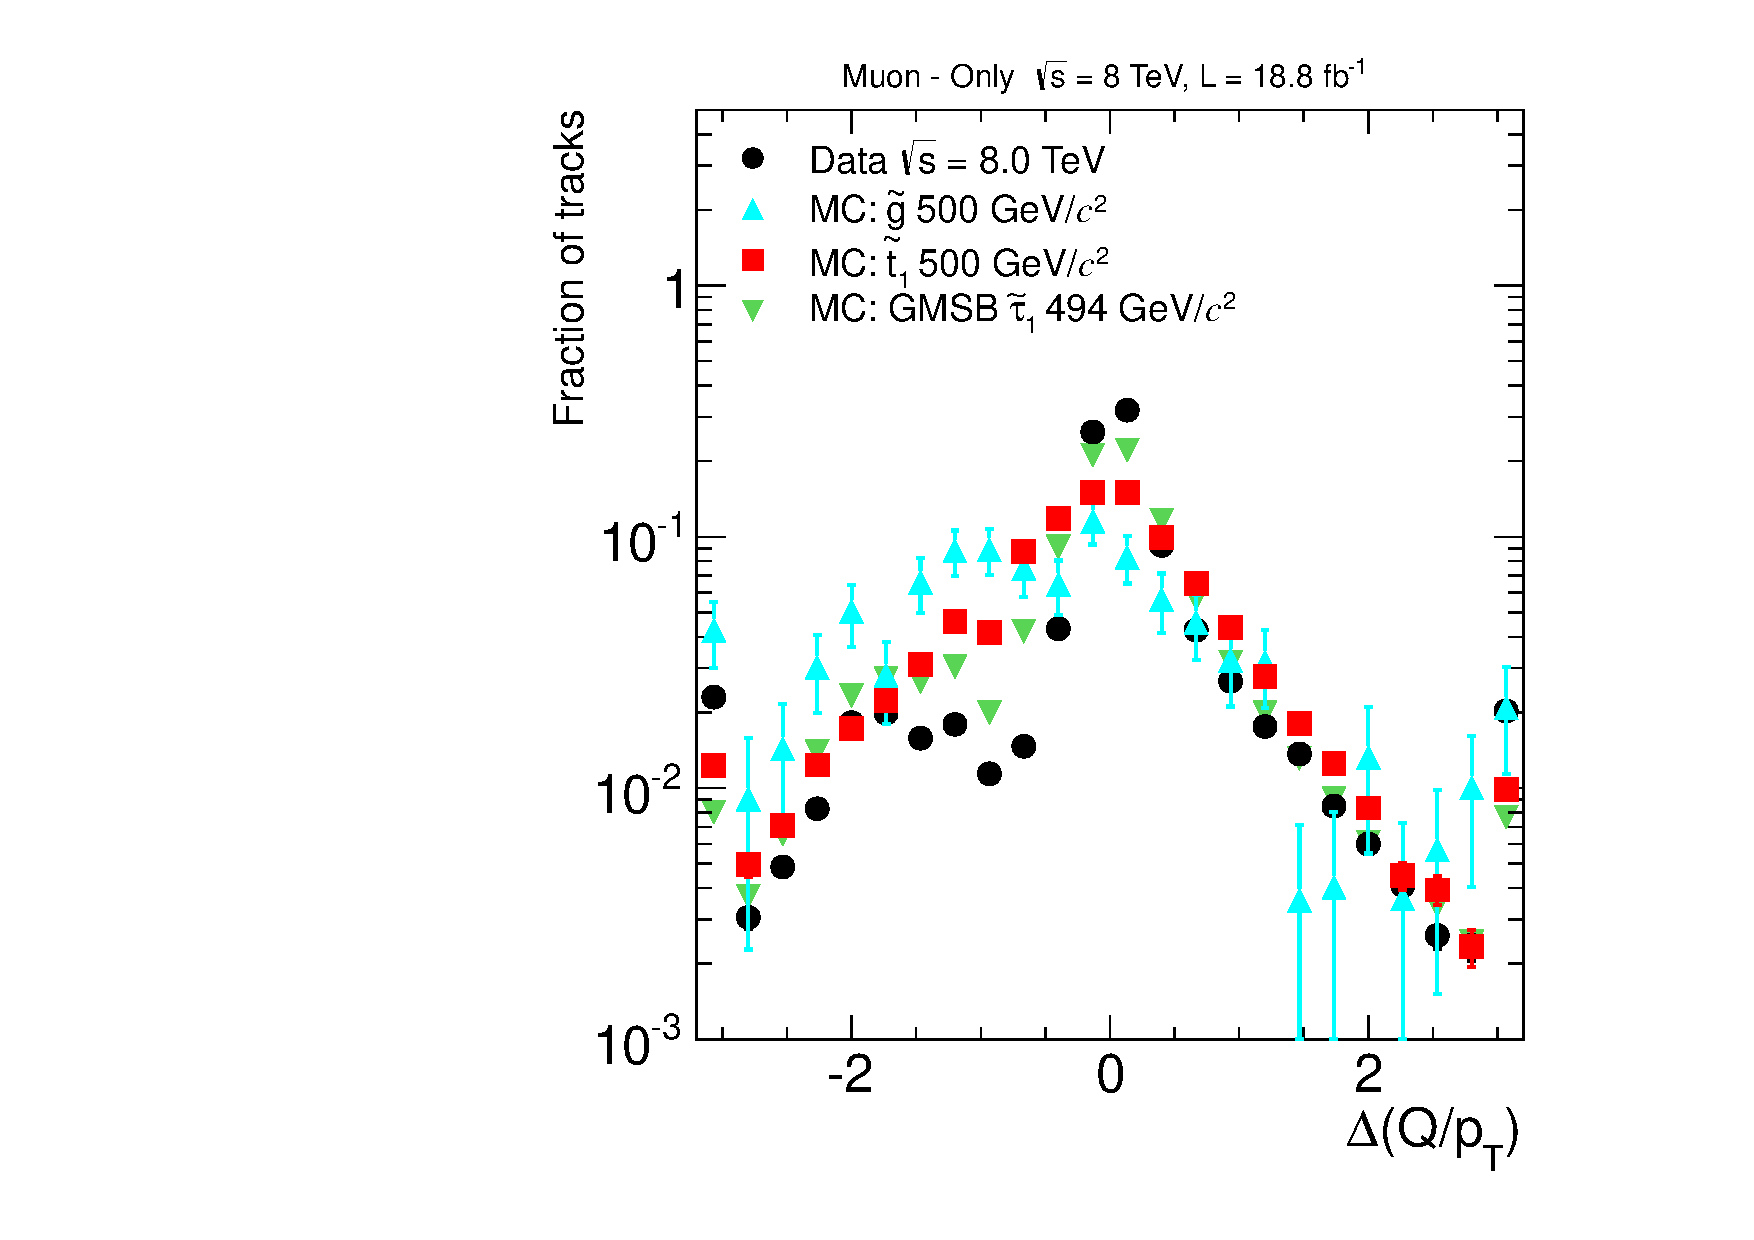
\includegraphics[width=0.44\textwidth]{figures/muonly/Selection_Comp_Signal_8TeV_InnerInvPtDiff_BS}
 \end{center}
 \caption{Distribution of $\Delta(Q/p_T)$
    for data, 500 GeV gluino, 500 GeV stop, and 494 GeV GMSB stau.
    \label{fig:MuOnlyInvPtDiff}}
\end{figure}

For the lepton like samples with non-unit charge, the \pt\ will be mismeasured by a factor of 1/Q, meaning multiply charged particles will have their \pt\ underestimated
This effect can be seen in Figure~\ref{fig:RecoGenPt}.
%For the lepton like samples with non-unit charge the \pt\ will be mismeasured by a factor of 1/Q, meaning fractionally charged particles will have their \pt\ overestimated
%while multiply charged particles will be underestimated. This effect can be seen in Figure~\ref{fig:RecoGenPt}.

\begin{figure}
 \begin{center}
  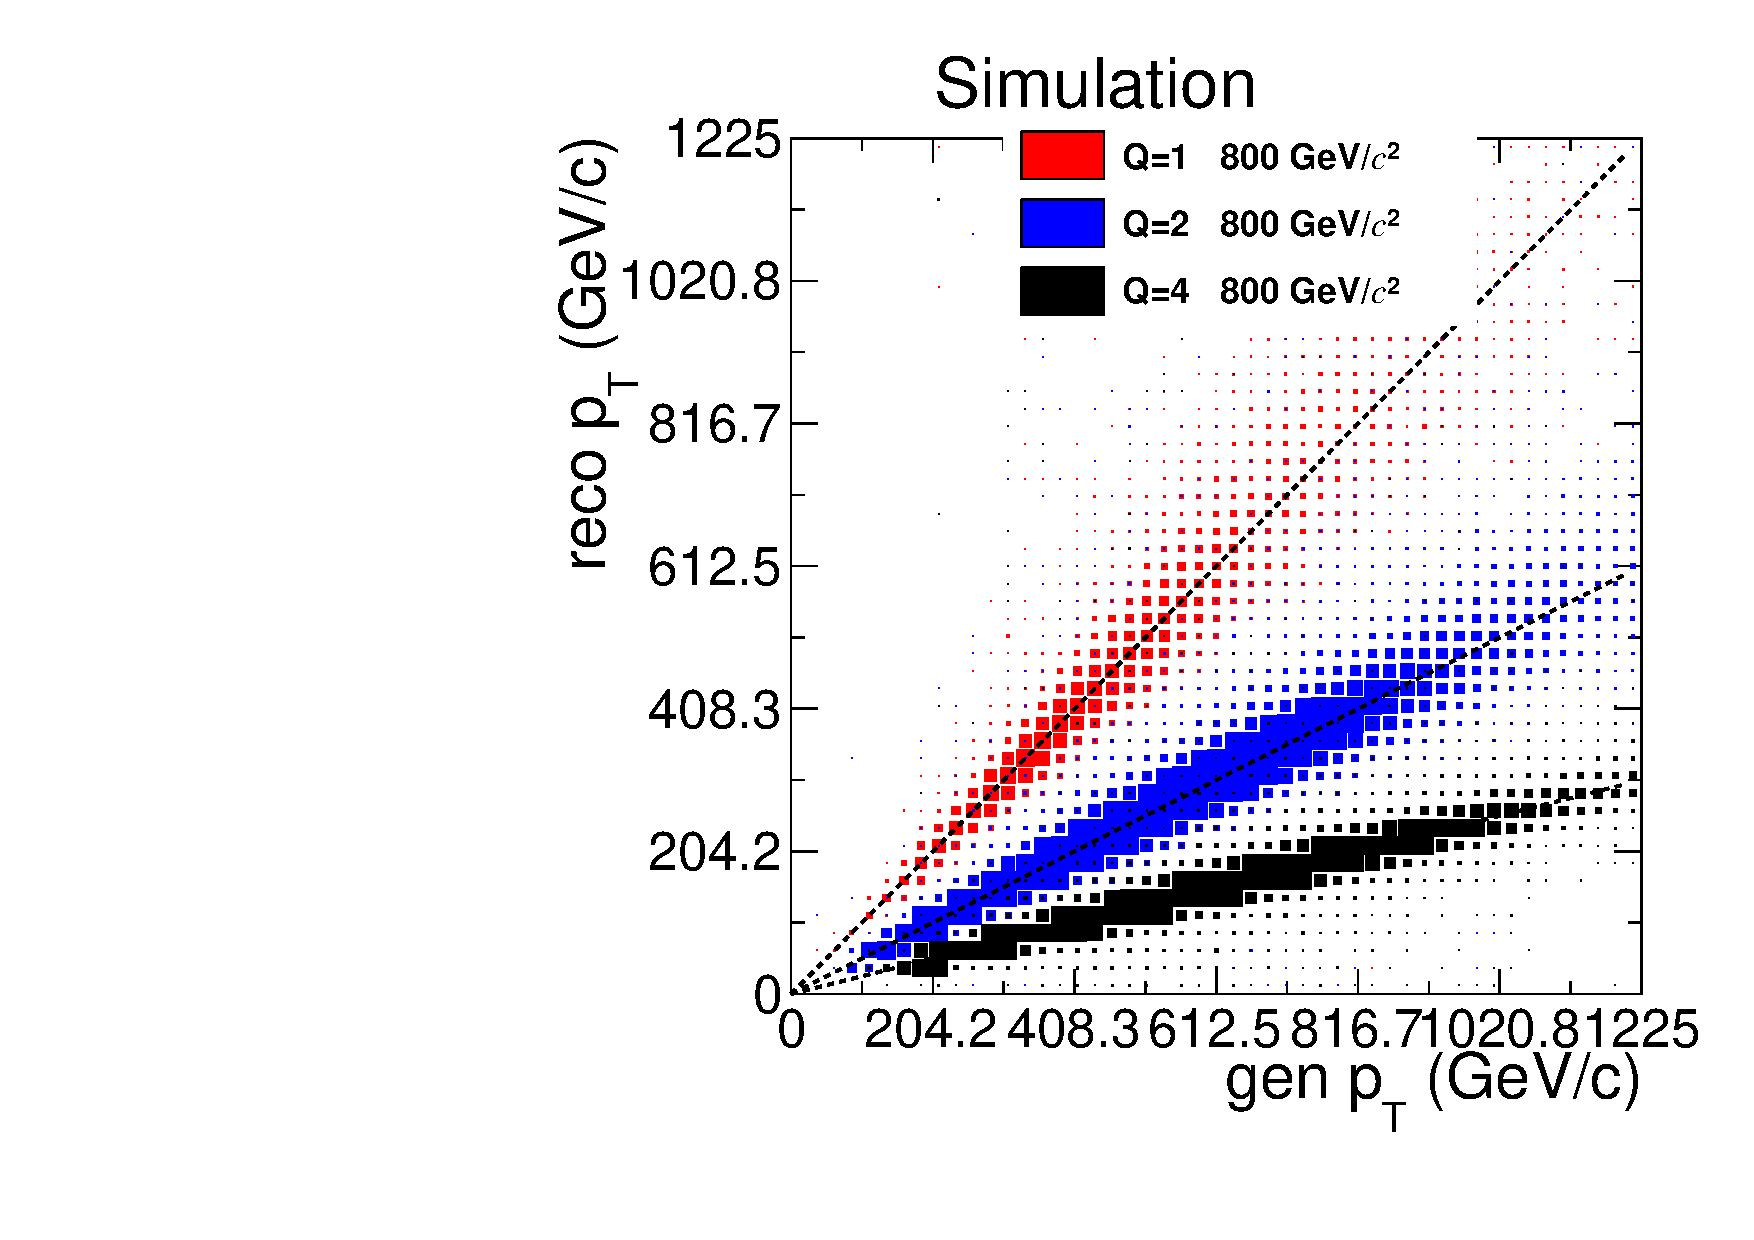
\includegraphics[width=0.44\textwidth]{figures/tkonly/SIM_Validation_Pt.pdf}
 \end{center}
 \caption{Distribution of reconstructed $p_T$ versus generator $p_T$ for Q=1e, 2e, and 4e samples.
    \label{fig:RecoGenPt}}
\end{figure}